\documentclass[sokoban_generation_thesis.tex]{subfiles}

Wszystkie eksperymenty zostały wykonane przy zachowaniu sugerowanych przez autorów wartości hiperparametrów algorytmu PPO2 \cite{sok_ppo}, które wymieniono w~tabeli \ref{tab:ppo_hyperparams}. Wartości nagród wypłacanych agentom również bazowały na~pracy \cite{sok_ppo}, co~wylistowano w~tabeli \ref{tab:ppo_reward_values}.

\begin{table}[h!]
	\smallskip
	\centering
	\caption{Użyte wartości hiperparametrów algorytmu PPO2}
	\label{tab:ppo_hyperparams}
	\begin{tabular}{|l|l|}
		\hline
		\textbf{Nazwa parametru} & \textbf{Wartość} \\
		\hline
		Gamma & 0.99\\
		Współczynnik entropii & 0.01\\
		Współczynnik uczenia & 0.00025 \\
		\hline
	\end{tabular}
\end{table}

\begin{table}[h!]
	\smallskip
	\centering
	\caption{Nagrody wypłacane agentom podczas procesu treningu}
	\label{tab:ppo_reward_values}
	\begin{tabular}{|l|l|}
		\hline
		\textbf{Typ} & \textbf{Wartość} \\
		\hline
		Poprawność poziomu & 5 \\
		Obecność gracza & 3 \\
		Poprawna liczba pudeł & 2 \\
		Poprawna liczba pól docelowych & 2 \\
		Poprawna proporcja pudeł & 2 \\
		Długość rozwiązania & 1 \\
		\hline
	\end{tabular}
\end{table}


\subsection{Poprawność plansz} \label{subs:ppo_poprawnosc}
Najistotniejszą różnicą między metodą PPO a~pozostałymi prezentowanymi, jest ryzyko generowania niepoprawnych plansz. Przez planszę poprawną rozumie się planszę spełniającą poniższe warunki.
\begin{itemize}
	\item Na~planszy znajduje się dokładnie jeden gracz.
	\item Liczba pudeł odpowiada liczbie pól docelowych.
	\item Istnieje sekwencja ruchów gracza, która przekształca daną planszę w~rozwiązaną planszę.
\end{itemize}

Wobec tego, istotne jest uczenie modeli generujących jak najwięcej poprawnych plansz, ponieważ tylko takie uznaje się za~użyteczne. Zbadano zależność poprawności generowanych poziomów od~liczby kroków agenta w~procesie uczenia. Wyniki tych badań zobrazowano na~rys.~\ref{rys:ppo_poprawnosc}. Jak widać, dla agentów opartych o~reprezentację wąską i~żółwią, po~wykonaniu stu milionów kroków poprawność utrzymuje się na~poziomie $80-85\%$. Taką liczbę kroków maszyna opisana w~rozdziale \ref{subs:test_pc} uzyskuje po~dziesięciu godzinach treningu. Bazując na~przeprowadzonych analizach, nie warto dalej trenować agentów opartych o~te~reprezentacje. Jednak w~przypadku reprezentacji szerokiej, między dziesiątą a~dziewiętnastą godziną treningu, średnia poprawność wzrosła z~$56\%$ do~$68\%$, zachowując wciąż tendencję rosnącą. Te~różnice można tłumaczyć przez większą przestrzeń dostępnych akcji reprezentacji szerokiej. Wyniki analiz pokryły się z~badaniami przedstawionymi w~\cite{sok_ppo}.

\begin{figure}[h]
	\centering
	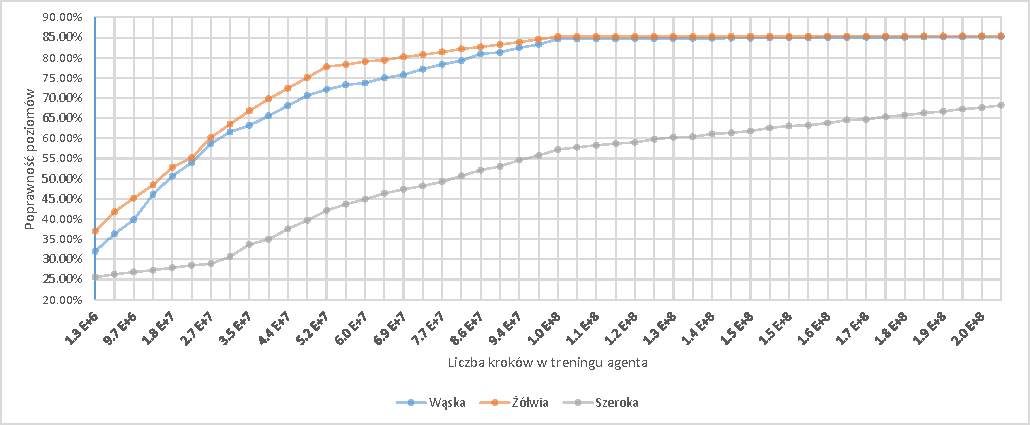
\includegraphics[width=0.9\textwidth]{wykres_ppo_poprawnosc}
	\caption{Zależność poprawności generowanych plansz od~liczby kroków uczenia}
	\label{rys:ppo_poprawnosc}
\end{figure}


\subsection{Wydajność czasowa treningu} \label{subs:ppo_time_training}
Opisywane w~p.~\ref{subs:ppo_poprawnosc} liczby kroków uczenia należy przełożyć na~czas w~celu zestawiania tej metody z~innymi. Średnia liczba kroków wykonywana w~jednostce czasu jest stała podczas całego procesu uczenia i~wynosi dla użytej maszyny $2777$ kroków na~sekundę. W~związku z~tym, uczenie agenta przez sto milionów kroków zajmuje niecałe dziesięć godzin, a~przez dwieście milionów kroków -- niespełna dziewiętnaście godzin. Przykłady plansz zewaluowanych dla agentów po~stu i~dwustu milionach kroków uczenia zaprezentowano odpowiednio na~rys.~\ref{rys:ppo_results_1} i~\ref{rys:ppo_results_2}.

\begin{figure}[h]
	\centering
	\begin{subfigure}[b]{0.3\linewidth}
		\centering
		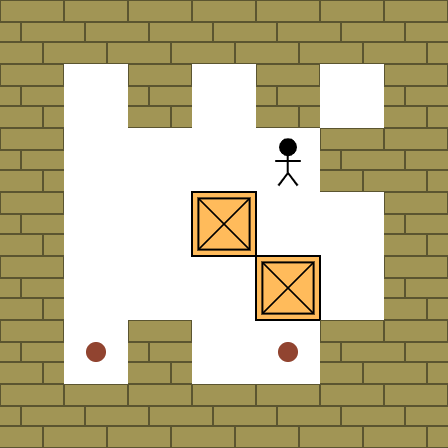
\includegraphics[width=0.7\linewidth]{board_ppo_turtle_1}
		\caption{Reprezentacja wąska}
	\end{subfigure}
	\begin{subfigure}[b]{0.3\linewidth}
		\centering
		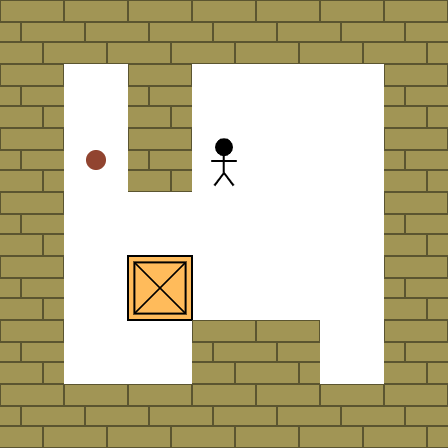
\includegraphics[width=0.7\linewidth]{board_ppo_narrow_1}
		\caption{Reprezentacja żółwia}
	\end{subfigure}
	\begin{subfigure}[b]{0.3\linewidth}
		\centering
		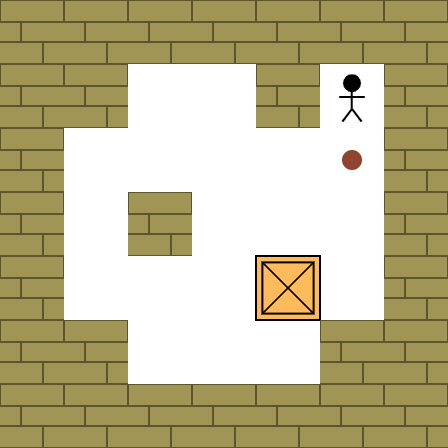
\includegraphics[width=0.7\linewidth]{board_ppo_wide_1}
		\caption{Reprezentacja szeroka}
	\end{subfigure}
	\caption{Plansze o~najwyższych wypłatach dla agenta uczonego przez $9$ godzin i~$30$ minut}
	\label{rys:ppo_results_1}
\end{figure}

\begin{figure}[h]
	\centering
	\begin{subfigure}[b]{0.3\linewidth}
		\centering
		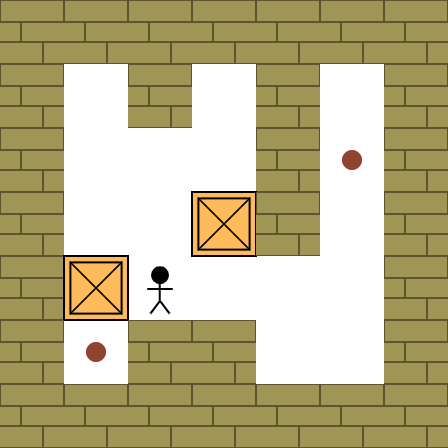
\includegraphics[width=0.7\linewidth]{board_ppo_turtle_2}
		\caption{Reprezentacja wąska}
	\end{subfigure}
	\begin{subfigure}[b]{0.3\linewidth}
		\centering
		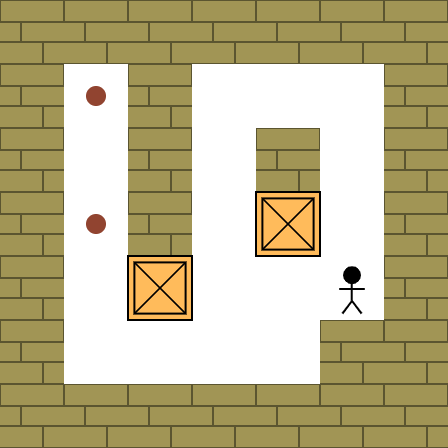
\includegraphics[width=0.7\linewidth]{board_ppo_narrow_2}
		\caption{Reprezentacja żółwia}
	\end{subfigure}
	\begin{subfigure}[b]{0.3\linewidth}
		\centering
		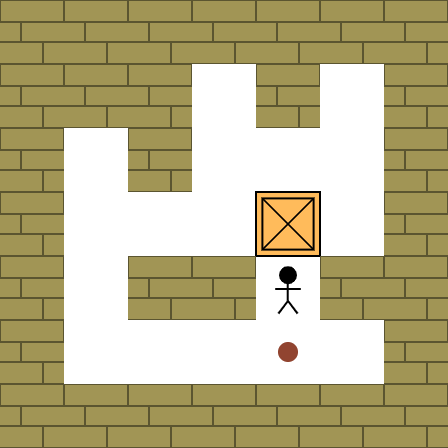
\includegraphics[width=0.7\linewidth]{board_ppo_wide_2}
		\caption{Reprezentacja szeroka}
	\end{subfigure}
	\caption{Plansze o~najwyższych wypłatach dla agenta uczonego przez $19$ godzin}
	\label{rys:ppo_results_2}
\end{figure}


\subsection{Wydajność czasowa ewaluacji} \label{subs:ppo_time}
W p.~\ref{subs:ppo_poprawnosc} zbadano zależność długości treningu od~poprawności generowanych plansz, wykazując że~zadowalającą poprawność (powyżej $50\%$) utrzymuje się po~około $110$ minutach treningu dla reprezentacji wąskiej i~żółwiej, a~dla szerokiej -- po~$470$. Jako że~proces generowania plansz metody PPO wymaga ewaluacji wyuczonego agenta, postanowiono zbadać również czas na~to~potrzebny. Wobec tego wybrano trzech najlepszych agentów wyuczonych w~trakcie eksperymentów dla różnych rozmiarów plansz i~wyznaczono średnią po~tysiąckrotnej ewaluacji. Jak widać w~tab.~\ref{tab:ppo_avg_inference_times}, średnie czasy nie przekraczają trzech sekund, a~dla najmniejszych plansz -- jednej.

\begin{table}[h!]
	\smallskip
	\centering
	\caption{Średnie czasy ewaluacji w~sekundach}
	\label{tab:ppo_avg_inference_times}
	\begin{tabular}{|l|l|l|l|}
		\hline
			\textbf{Rozmiar} & \textbf{Wąska} & \textbf{Żółwia} & \textbf{Szeroka} \\
			\hline
			4& 0.2& 0.1& 0.1\\
			5& 0.2& 0.3& 0.3\\
			6& 0.8& 0.6& 0.6\\
			7& 1.4& 1.3& 1.2\\
			8& 2.3& 2.0& 2.0\\
			9& 2.2& 2.9& 1.3\\            
		\hline
	\end{tabular}
\end{table}

Mimo iż~średnie czasy ewaluacji wydają się być niskie, to~metoda nie daje gwarancji tak szybkiej ewaluacji, co~ukazano w~tab.~\ref{tab:ppo_max_inference_times}. Maksymalne czasy ewaluacji dla większych plansz (o rozmiarach $8$ i~$9$) przekraczały $10$ sekund, w~jednym przypadku sięgając nawet $19.4$ s.~Niższe wartości średnie i~maksymalne w~przypadku reprezentacji szerokiej spowodowane są~niższym skomplikowaniem generowanych plansz, które są~szybciej weryfikowane przez \textit{solver}.


\begin{table}[h!]
	\smallskip
	\centering
	\caption{Maksymalne czasy ewaluacji w~sekundach}
	\label{tab:ppo_max_inference_times}
	\begin{tabular}{|l|l|l|l|}
		\hline
		\textbf{Rozmiar} & \textbf{Wąska} & \textbf{Żółwia} & \textbf{Szeroka} \\
		\hline
		4& 0.2& 0.2& 0.3\\
		5& 1.2& 3.4& 0.6\\
		6& 2.2& 1.6& 0.7\\
		7& 8.6& 5.9& 5.6\\
		8& 19.4& 9.6& 7.3\\
		9& 15.2& 12.7& 10.9\\            
		\hline
	\end{tabular}
\end{table}


\subsection{Sumaryczna wydajność czasowa}
W celu podsumowania p.~\ref{subs:ppo_time_training} i~\ref{subs:ppo_time}, zbadano ile czasu potrzeba dla każdej reprezentacji, by~osiągnąć poprawną planszę $5$x$5$ z~prawdopodobieństwem odpowiednio $50\%$, $65\%$ i~$75\%$. Analizowano sumę czasu treningu i~ewaluacji. Z~wyników analizy zaprezentowanych na~rys.~\ref{rys:ppo_czas_total} wnioskuje się, że~aby uzyskać z~$50\%$ szansą poprawny poziom $5$x$5$ dla reprezentacji żółwiej i~wąskiej, potrzeba mniej niż dwóch godzin, a~dla reprezentacji szerokiej -- ponad osiem godzin pracy metody. 

\begin{figure}[h]
	\centering
	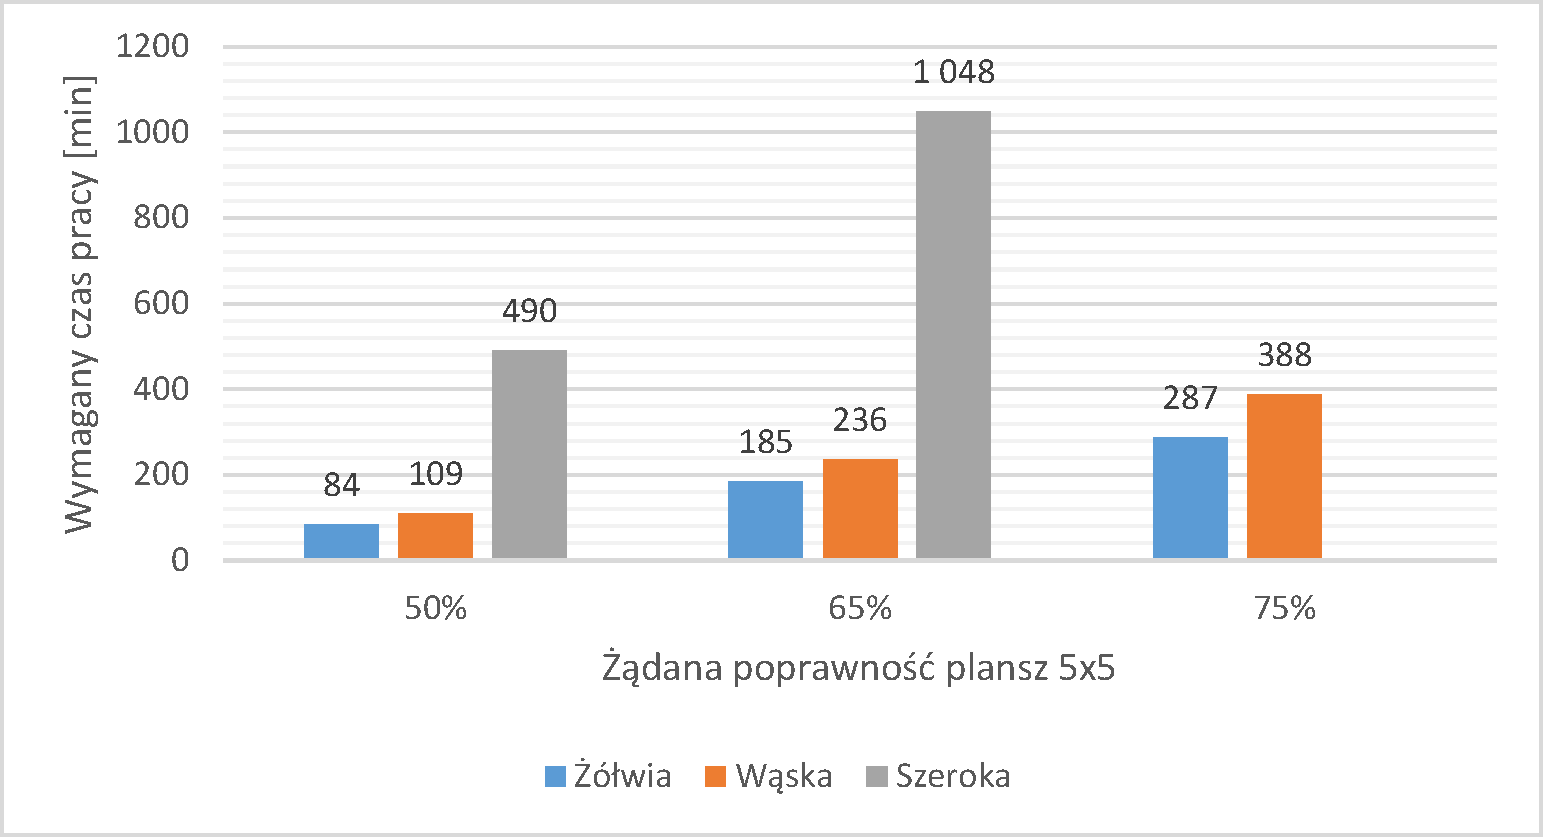
\includegraphics[width=0.8\textwidth]{ppo_czas_total}
	\caption{Zależność czasu pracy metody od~żądanej poprawności}
	\label{rys:ppo_czas_total}
\end{figure}


\subsection{Nagrody}
W celu zbadania tempa uczenia, przeanalizowano uśrednione wypłaty dla agentów podczas procesu treningu. Na~wyniki testów ukazane na~rys.~\ref{rys:ppo_avg_reward_trend} nałożono linie trendu, które potwierdzają hipotezę z~rozdziału \ref{subs:ppo_poprawnosc} o~wciąż trwającym procesie poprawy agentów z~reprezentacją szeroką.

\begin{figure}[h!]
	\centering
	\begin{subfigure}[b]{\linewidth}
		\centering
		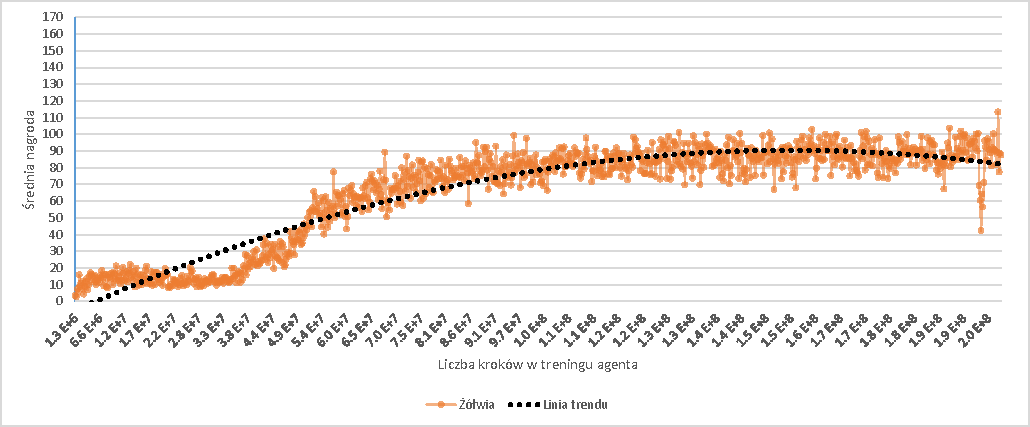
\includegraphics[width=0.9\textwidth]{wykres_nagroda_zolwia}
	\end{subfigure}
	\begin{subfigure}[b]{\linewidth}
		\centering
		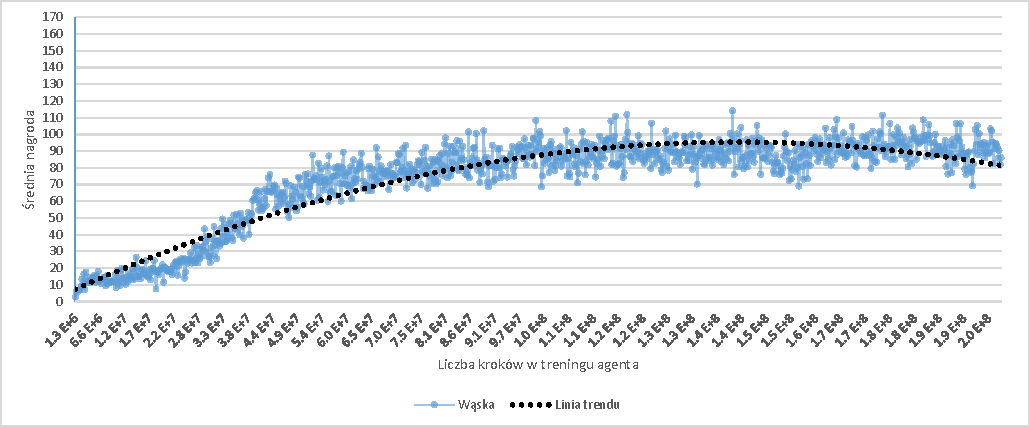
\includegraphics[width=0.9\textwidth]{wykres_nagroda_waska}
	\end{subfigure}
	\begin{subfigure}[b]{\linewidth}
		\centering
		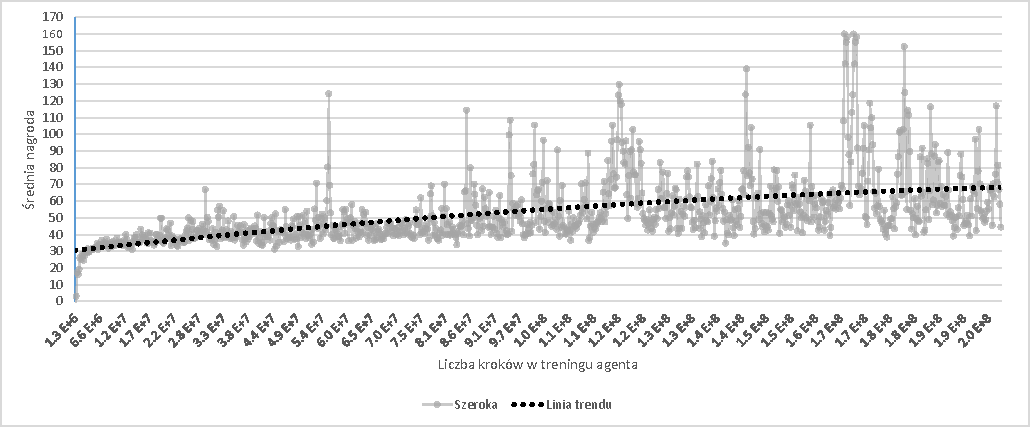
\includegraphics[width=0.9\textwidth]{wykres_nagroda_szeroka}
	\end{subfigure}
	\caption{Zależność średniej nagrody od~liczby kroków uczenia}
	\label{rys:ppo_avg_reward_trend}
\end{figure}

Podczas badania średnich nagród w~procesie uczenia zauważono również, iż~ich rozkład jest zmienny w~różnych etapach uczenia dla różnych reprezentacji. Po~podzieleniu procesu uczenia na~cztery równe fazy, stworzono wykres zmienności rozkładu średnich nagród z~rys.~\ref{rys:ppo_rozklad_nagrod}. Jak widać, reprezentacja wąska i~żółwia stabilizuje się w~późniejszych fazach, zawężając tym samym rozkład otrzymywanych nagród. Reprezentacja szeroka, mimo tendencji wzrostowych, otrzymuje w~każdej fazie coraz szerszy przedział średnich wypłat.

\begin{figure}[h!]
	\centering
	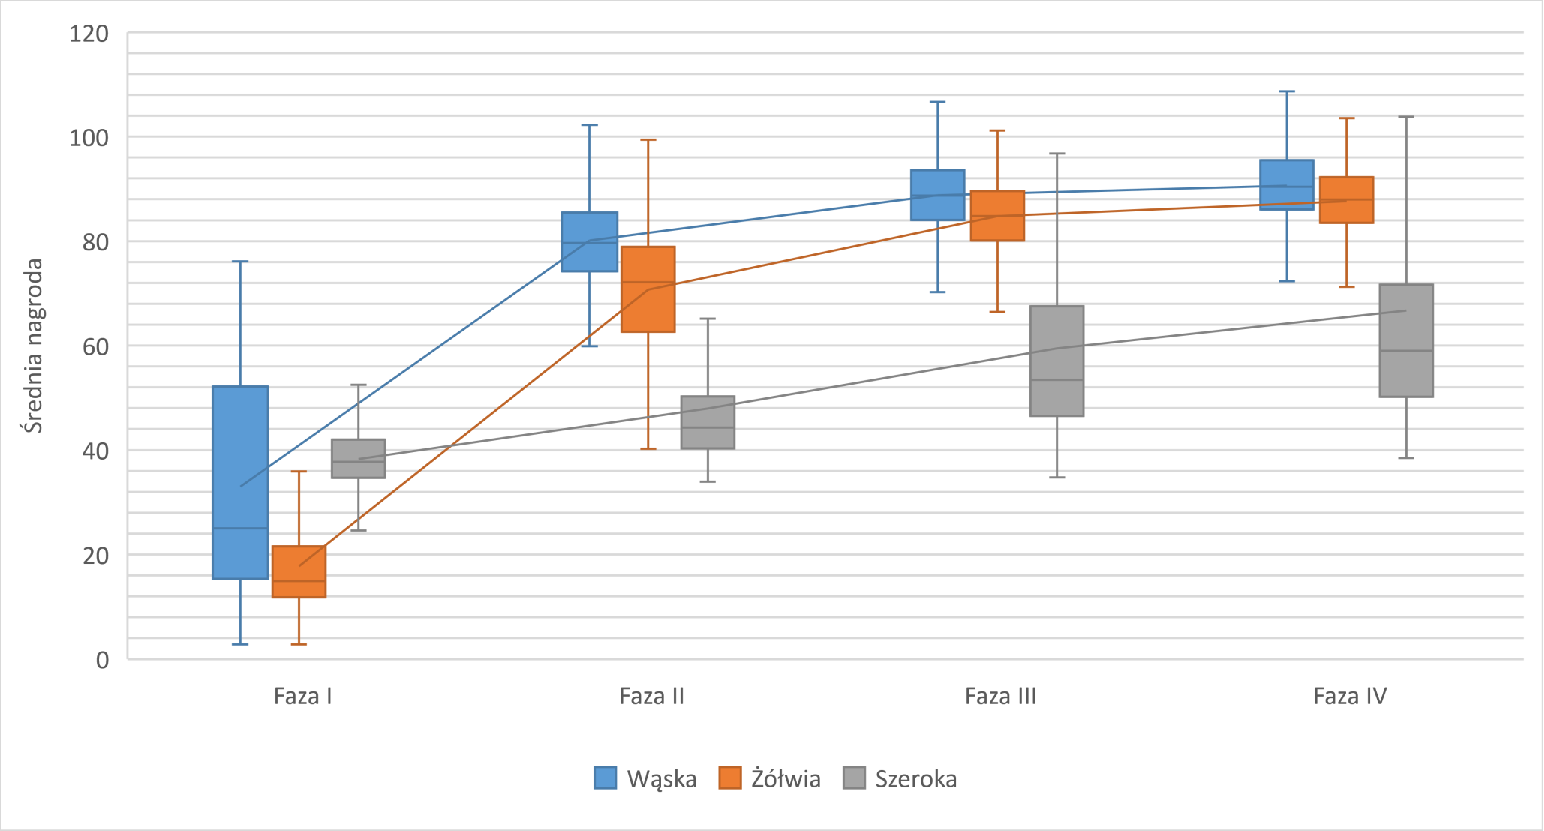
\includegraphics[width=0.8\textwidth]{wykres_ppo_rozklad_nagrod}
	\caption{Rozkład średnich nagród w~poszczególnych fazach uczenia}
	\label{rys:ppo_rozklad_nagrod}
\end{figure}



\subsection{Rozmiar planszy}
Wszystkie poprzednio opisane eksperymenty generowały plansze o~rozmiarze $5x5$. Postanowiono jednak zbadać, jak metoda PPO radzi sobie z~planszami większych rozmiarów. W~tym celu wytrenowano dodatkowo osiemnastu agentów, z~limitem na~czas uczenia równym osiem godzin. Dla sześciu różnych rozmiarów plansz i~trzech różnych reprezentacji dokonano później wielokrotnej ewaluacji w~celu sprawdzenia średniej poprawności. Wyniki tego eksperymentu, ukazane na~rys.~\ref{rys:ppo_rozmiar}, jasno wskazują na~to, że~metoda nie nadaje się dla plansz o~rozmiarach większych niż $7x7$.

\begin{figure}[h!]
	\centering
	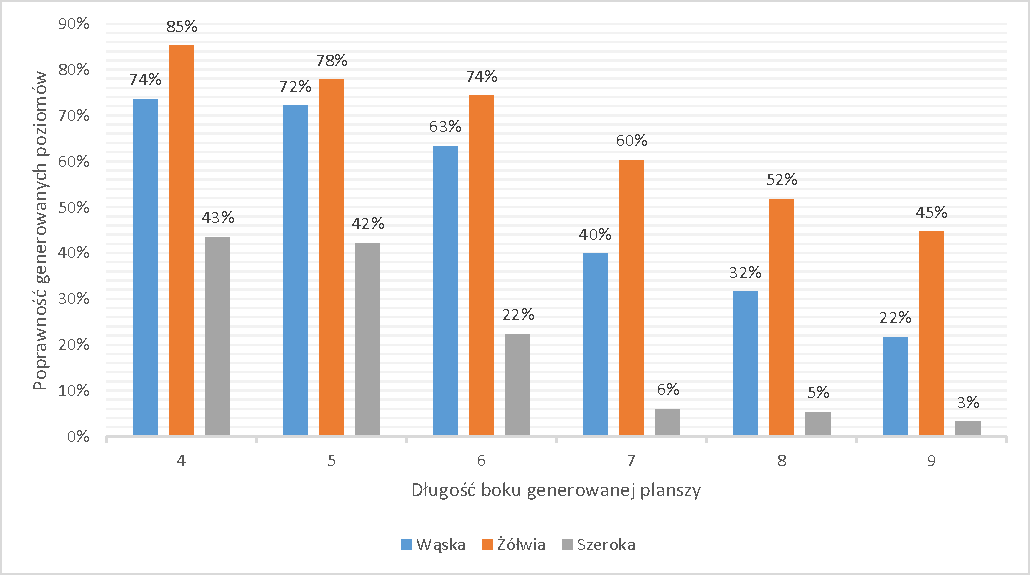
\includegraphics[width=0.8\textwidth]{wykres_ppo_rozmiar}
	\caption{Zależność poprawności generowanych plansz od~długości boku}
	\label{rys:ppo_rozmiar}
\end{figure}
